

\section{Teknisk bakgrund}
Detta kapitel ger en teoretisk översikt över de grundläggande komponenterna i larmsystem, och hur de fungerar. I samband med detta förklaras en del av hårdvaran som används i projektet ingående. Efter det beskrivs teorin bakom kommunikationstandarden CAN. 
\label{sec:tekniskbakgrund}
\subsection{Larmsystem}
Larmsystem kan variera när det gäller utrustning och komplexitet, men det finns gemensamma komponenter som utgör en bas för systemen. Denna bas består ofta av \textit{sensorer}, \textit{centralutrustning} och \textit{larmdon} \cite[s. 15]{lundh:2008}.  
%REFERERA TILL DENNA BOK IST
%VAD GÖR MAN OM BOKEN HAR ETT ANNAT ORD FÖR CENTRALENHET
%https://www.bokus.com/bok/9789188816108/larm-overvaknings-och-sakerhetssystem-faktabok/
Sensorerna är larmsystemets ''sinnen''. Deras uppgift är att upptäcka ändringar i tillstånd. Tillstånden kan vara tryck, ljud, ljus, slutande eller brytande kontakt, \cite[s. 15]{lundh:2008}. 
Denna ändring i tillstånd signaleras till centralutrustningen genom systemets kommunikationsstandard. Ett gemensamt kommunikationsprotokoll används för det valda mediet. \newline \newline 
Om sensorerna är larmsystemets ''sinnen'' är centralutrustningen larmsystemets ''hjärna''. Centralenheten tar emot information från sensorerna, och dess uppgift är att tolka vad denna information betyder \cite[s. 18]{lundh:2008}. När centralenheten har tolkat informationen bestämmer den vad som ska göras härnäst. Om någon av sensorerna har gett ett oroväckande utslag kanske centralenheten skickar en signal till ett larmdon. 

\subsection{Projektets kommunikationstandard, CAN}
\label{sec:can}
CAN, Controller Area Network, är en databuss som utvecklades för fordonsindustrin. Denna buss tillåter kommunikation mellan flera enheter, där alla enheter delar samma kommunikationsmedium. Protokollet har också förmågan att självdiagnostisera och reparera fel i meddelanden. \begin{flushright}
\cite[s. 2]{corrigan:2016}
\end{flushright} 
För att förhindra och alternativt optimera kollisioner använder sig CAN av protokollet CSMA/CD+AMP. Detta protokoll gör så att noder ''lyssnar innan de pratar'', de väntar en specificerad tid innan de börja sända information. Om en kollision skulle uppstå används meddelandenas prioritet för att lösa den – meddelandet med högre prioritet fortsätter att sända. När ett larmsystem utvecklas kan detta användas till systemets fördel; utvecklare kan definera att larmmeddelanden alltid har högsta prioritet. \begin{flushright}
\cite[s. 3]{corrigan:2016}
\end{flushright} 

CAN-meddelanden är förpackade i så kallade CAN-ramar och har en standardiserad struktur. Den CAN-ram som anses vara av standardstruktur visualiseras i figur \ref{fig:can_frame}. Diverse fält i ramen beskrivs nedan:
\begin{description}
    \item[ID-fältet] {Innehåller meddelandets ID.}
    \item[Reserverat] {Innehåller information angående vad för typ av ram det är samt vilket typ av ID ramen använder sig av.}
    \item[Längd] {Längden på databufferten i bytes.}
    \item[Data Buffert] {Bufferten där all data ligger. Längd-fältet beskriver databuffertens storlek.}
    \item[CRC-fältet] {\emph{Cyclic Redundancy Check} är en felkontrollskod. Den används för att undersöka om ett meddelande har kommit fram oskadat.}
    \item[ACK] {\emph{Acknowledge} skickas av mottagande noder för att tala om för avsändarnoden att meddelandet kom fram. }
\end{description}
\begin{figure}[h]
    \centering
    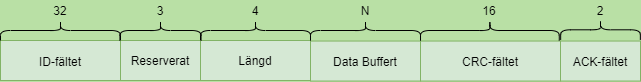
\includegraphics[scale=0.52]{dokumentation/projektrapport/IMAGES/can_frame.png}
    \caption{En CAN-ram av standardstruktur. Talen beskriver antalet bytes. N innebär att databuffertens längd kan variera. Den bestäms av värdet i längd-fältet.}
    \label{fig:can_frame}
\end{figure}


\subsection{Projektets sensortyper}
\label{sec:sensortyper}
%I detta projekt används tre typer av sensorer: magnetkontakter, %vibrationssensorer och avståndssensorer. Magnetkontakten som används %består av två delar: en magnet och en mekanisk kontakt. Om kontakten %är kopplad till en elektrisk krets hålls kretsen sluten, så länge %magneten är nära den (Nästan så de vidrör varandra). Denna sensor %fungerar utan någon strömtillförsel. [a.a] I projektet tillämpas %denna funktion i dörrenheten.
I detta projekt används tre typer av sensorer: en magnetkontakt, en vibrationssensor och en avståndssensor. Magnetkontakten som används består av två delar: en magnet och en mekanisk kontakt. Kontakten påverkas av magnetens fält, och om denna är kopplad till en elektrisk krets, kan denna krets slutas eller brytas \cite[s. 15]{lundh:2008}. Så länge magneten är nära kontakten hålls kretsen sluten, och sensorn behöver ingen strömförsörjning för att detta ska fungera. Det här används för att kontrollera om en dörr är stängd. 
\newline \newline
Till skillnad från magnetkontakten behöver resten av sensorerna strömförsörjning.
Vibrationssensorn som används kallas \textit{SW-18010P}. Sensorn har en liten fjäder innanför sitt metallskal, och när denna fjäder vidrör skalet sluts kretsen. Den reagerar därför på rörelse och vibration från alla möjliga riktningar. I projektet används det för att detektera inbrott, t.ex. att en ruta krossas.
Avståndssensorn \textit{HC-SR04} använder ultraljud för att rapportera hur nära något är i dess synfält. Sensorn avger ultraljudsvågor, och mäter hur lång tid det tar dem att komma tillbaka. Tiden och frekvensen av vågorna används för att uppskatta hur långt de färdades. Den kan mäta avstånd från 2 till 400 centimeter med upp till tre millimeter exakthet, och används för att detektera om någon eller något närmar sig. 
\begin{flushright} 
\cite{elecfreaks} , \cite{bailing:2011}
\end{flushright}



\newpage
\subsection{MD407 - En översikt}
\label{sec:md407}
Mikrokontrollern MD407 har många anslutningsportar på sitt kretskort. Här beskrivs de portarna som är relevanta för projektet, och var de befinner sig (se figur \ref{fig:md407}).

\begin{figure}[h]
    \begin{center} 
    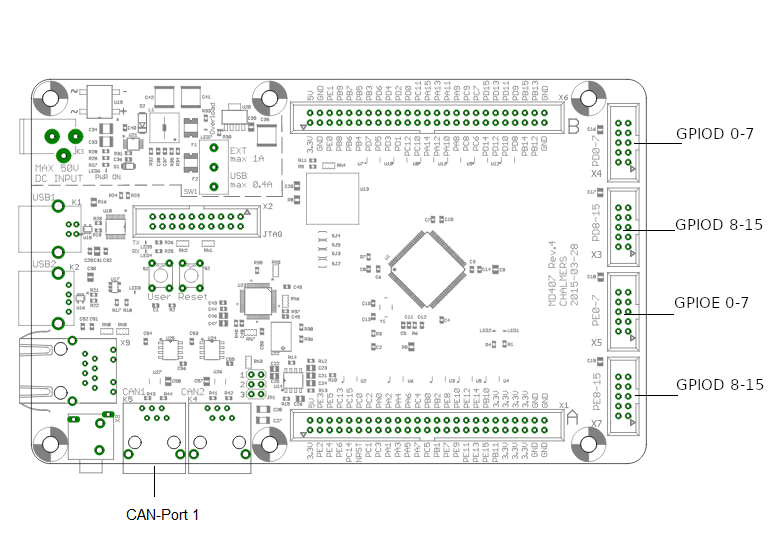
\includegraphics[scale=0.55]{dokumentation/projektrapport/IMAGES/md407.png}
    \caption{Portar på MD407 som är relevanta för projektet. De gröna cirklarna inuti GPIO-portarna representerar en anslutningspunkt, där en kabel kan anslutas. En anslutningspunkt kan beskrivas som en ''pin'' \cite{md407}.}
    \label{fig:md407}
    \end{center} 
    ''CAN-port 1'' används för att koppla samtliga enheter till CAN-bussen. GPIO-portarnas nummer refererar till vilka ''pinnar'' portarna har: GPIOD 0-7 har pinnar 0-7.
\end{figure}
\newpage